\documentclass[a4paper,11pt]{article}
\usepackage[margin=2.5cm]{geometry}
\usepackage[authoryear,round]{natbib}
\let\cite\citep
\usepackage{graphicx}
\usepackage{booktabs}
\usepackage{array}
\usepackage{tabularx}
\usepackage{longtable}
\usepackage{xspace}
\usepackage{xcolor}
\usepackage[colorlinks=true,allcolors={blue!60!black}]{hyperref}
%% Dibuat otomatis oleh tools/scopus/angka_naskah.py; jangan disunting manual.
%% Setiap makro adalah satu angka korpus yang dihitung dari literature/scopus-2026-09.
\newcommand{\kHumElig}{0.45\xspace}
\newcommand{\kHumTitles}{0.57\xspace}
\newcommand{\nAbsIncl}{1{,}013\xspace}
\newcommand{\nApp}{64\xspace}
\newcommand{\nAppOnly}{0\xspace}
\newcommand{\nAppTrack}{57\xspace}
\newcommand{\nAppWith}{64\xspace}
\newcommand{\nAssessed}{1{,}145\xspace}
\newcommand{\nAwaiting}{0\xspace}
\newcommand{\nClassAfter}{3\xspace}
\newcommand{\nClassDuring}{10\xspace}
\newcommand{\nClassPerDet}{1\xspace}
\newcommand{\nClassSingle}{33\xspace}
\newcommand{\nClassSingleBlueberry}{5\xspace}
\newcommand{\nClassSingleMaturity}{28\xspace}
\newcommand{\nClassSingleTomato}{10\xspace}
\newcommand{\nClassUnstated}{14\xspace}
\newcommand{\nClassVote}{5\xspace}
\newcommand{\nCodedAbs}{0\xspace}
\newcommand{\nCodedFull}{240\xspace}
\newcommand{\nCodedTitle}{0\xspace}
\newcommand{\nCombined}{95\xspace}
\newcommand{\nCropApple}{71\xspace}
\newcommand{\nCropCitrus}{28\xspace}
\newcommand{\nCropGrape}{24\xspace}
\newcommand{\nCropMango}{15\xspace}
\newcommand{\nCropStrawberry}{13\xspace}
\newcommand{\nCropTomato}{31\xspace}
\newcommand{\nDepth}{94\xspace}
\newcommand{\nDepthApple}{33\xspace}
\newcommand{\nDepthLidar}{6\xspace}
\newcommand{\nDepthRgbd}{62\xspace}
\newcommand{\nDepthStereo}{13\xspace}
\newcommand{\nDiscrete}{30\xspace}
\newcommand{\nDiscreteGeom}{15\xspace}
\newcommand{\nDiscreteStat}{15\xspace}
\newcommand{\nDocType}{166\xspace}
\newcommand{\nEarly}{15\xspace}
\newcommand{\nEarlyGeom}{11\xspace}
\newcommand{\nEarlyStat}{4\xspace}
\newcommand{\nEarlyTrack}{2\xspace}
\newcommand{\nEligExcl}{132\xspace}
\newcommand{\nExclEight}{0\xspace}
\newcommand{\nExclFive}{60\xspace}
\newcommand{\nExclFour}{1\xspace}
\newcommand{\nExclOne}{23\xspace}
\newcommand{\nExclSeven}{1\xspace}
\newcommand{\nExclSix}{4\xspace}
\newcommand{\nExclThree}{25\xspace}
\newcommand{\nExclTwo}{18\xspace}
\newcommand{\nFTAssessed}{845\xspace}
\newcommand{\nFTExcl}{26\xspace}
\newcommand{\nFTExclEight}{2\xspace}
\newcommand{\nFTExclFive}{12\xspace}
\newcommand{\nFTExclFour}{0\xspace}
\newcommand{\nFTExclOne}{1\xspace}
\newcommand{\nFTExclSeven}{0\xspace}
\newcommand{\nFTExclSix}{0\xspace}
\newcommand{\nFTExclThree}{2\xspace}
\newcommand{\nFTExclTwo}{9\xspace}
\newcommand{\nFullText}{819\xspace}
\newcommand{\nGeom}{99\xspace}
\newcommand{\nGeomOnly}{66\xspace}
\newcommand{\nHumElig}{165\xspace}
\newcommand{\nHumEligAgree}{86\xspace}
\newcommand{\nHumTitles}{300\xspace}
\newcommand{\nHumTitlesAgree}{256\xspace}
\newcommand{\nIdentTermMax}{33\xspace}
\newcommand{\nIdentTermMin}{24\xspace}
\newcommand{\nIncluded}{819\xspace}
\newcommand{\nKelasBanding}{7\xspace}
\newcommand{\nKelasLain}{15\xspace}
\newcommand{\nKelasLainTengah}{9\xspace}
\newcommand{\nKelasLebih}{6\xspace}
\newcommand{\nKelasTengah}{11\xspace}
\newcommand{\nKelasTiga}{21\xspace}
\newcommand{\nKelasUnik}{6\xspace}
\newcommand{\nKelasUnikMentah}{3\xspace}
\newcommand{\nKelasUnikTengah}{2\xspace}
\newcommand{\nLearn}{8\xspace}
\newcommand{\nLearnOnly}{0\xspace}
\newcommand{\nLinks}{289\xspace}
\newcommand{\nMetCount}{197\xspace}
\newcommand{\nMetCountOnly}{52\xspace}
\newcommand{\nMetDet}{163\xspace}
\newcommand{\nMetIdent}{77\xspace}
\newcommand{\nMetNone}{6\xspace}
\newcommand{\nMethod}{235\xspace}
\newcommand{\nMethodMetric}{235\xspace}
\newcommand{\nModLidar}{10\xspace}
\newcommand{\nModMulti}{5\xspace}
\newcommand{\nModRgb}{190\xspace}
\newcommand{\nModRgbd}{18\xspace}
\newcommand{\nModStereo}{8\xspace}
\newcommand{\nMulti}{240\xspace}
\newcommand{\nMultiData}{5\xspace}
\newcommand{\nMultiEarlyMax}{9\xspace}
\newcommand{\nMultiFullText}{240\xspace}
\newcommand{\nMultiNoFullText}{0\xspace}
\newcommand{\nMultiPeak}{55\xspace}
\newcommand{\nMultiScopus}{239\xspace}
\newcommand{\nNoAbstract}{254\xspace}
\newcommand{\nNone}{1\xspace}
\newcommand{\nNoneOnly}{1\xspace}
\newcommand{\nNotRetrieved}{173\xspace}
\newcommand{\nNotRetrievedClass}{12\xspace}
\newcommand{\nNotRetrievedDepth}{30\xspace}
\newcommand{\nNotRetrievedMulti}{1\xspace}
\newcommand{\nNotRetrievedPalm}{48\xspace}
\newcommand{\nNotRetrievedReview}{17\xspace}
\newcommand{\nNotRetrievedSingle}{60\xspace}
\newcommand{\nNotRetrievedTransfer}{5\xspace}
\newcommand{\nOther}{5\xspace}
\newcommand{\nOtherComb}{16\xspace}
\newcommand{\nOtherRetrieved}{5\xspace}
\newcommand{\nOutside}{83\xspace}
\newcommand{\nPalm}{122\xspace}
\newcommand{\nPalmCls}{57\xspace}
\newcommand{\nPalmCount}{3\xspace}
\newcommand{\nPalmData}{4\xspace}
\newcommand{\nPalmDet}{22\xspace}
\newcommand{\nPalmField}{19\xspace}
\newcommand{\nPalmGround}{9\xspace}
\newcommand{\nPalmInstClass}{97\xspace}
\newcommand{\nPalmLoose}{4\xspace}
\newcommand{\nPalmMill}{40\xspace}
\newcommand{\nPalmMixed}{5\xspace}
\newcommand{\nPalmOnTree}{17\xspace}
\newcommand{\nPalmQual}{16\xspace}
\newcommand{\nPalmSensor}{16\xspace}
\newcommand{\nPalmUav}{2\xspace}
\newcommand{\nPalmUnstated}{22\xspace}
\newcommand{\nPalmViews}{17\xspace}
\newcommand{\nPalmWeb}{8\xspace}
\newcommand{\nPerClass}{33\xspace}
\newcommand{\nPlatGround}{91\xspace}
\newcommand{\nPlatHand}{52\xspace}
\newcommand{\nPlatLab}{1\xspace}
\newcommand{\nPlatNone}{38\xspace}
\newcommand{\nPlatSeveral}{16\xspace}
\newcommand{\nPlatUav}{32\xspace}
\newcommand{\nRecent}{155\xspace}
\newcommand{\nRefAnnot}{143\xspace}
\newcommand{\nRefHarvest}{43\xspace}
\newcommand{\nRefNone}{23\xspace}
\newcommand{\nRefPack}{2\xspace}
\newcommand{\nRefTree}{56\xspace}
\newcommand{\nRetrieved}{6{,}491\xspace}
\newcommand{\nReviews}{105\xspace}
\newcommand{\nRevisit}{5\xspace}
\newcommand{\nSampleTitles}{300\xspace}
\newcommand{\nSampleTitlesEligible}{11\xspace}
\newcommand{\nScan}{41\xspace}
\newcommand{\nScopusIncl}{814\xspace}
\newcommand{\nSingle}{142\xspace}
\newcommand{\nSingleView}{0\xspace}
\newcommand{\nSought}{1{,}018\xspace}
\newcommand{\nStat}{22\xspace}
\newcommand{\nStatOnly}{19\xspace}
\newcommand{\nTermCounting}{363\xspace}
\newcommand{\nTermDetection}{495\xspace}
\newcommand{\nTerms}{42\xspace}
\newcommand{\nTitleExcl}{4{,}578\xspace}
\newcommand{\nTitleRecheck}{1{,}325\xspace}
\newcommand{\nTitleReinstated}{19\xspace}
\newcommand{\nTitles}{5{,}723\xspace}
\newcommand{\nTrack}{141\xspace}
\newcommand{\nTrackGeom}{22\xspace}
\newcommand{\nTrackGeomScan}{7\xspace}
\newcommand{\nTrackGeomVideo}{15\xspace}
\newcommand{\nTrackOnly}{54\xspace}
\newcommand{\nUnique}{5{,}889\xspace}
\newcommand{\nVideo}{159\xspace}
\newcommand{\nWithAbstract}{665\xspace}
\newcommand{\nYearFirst}{8\xspace}
\newcommand{\nYearPeak}{140\xspace}
\newcommand{\pApp}{27}
\newcommand{\pAppRecent}{33}
\newcommand{\pGeom}{42}
\newcommand{\pHumElig}{52}
\newcommand{\pHumTitles}{85}
\newcommand{\pLearn}{3}
\newcommand{\pMetCount}{84}
\newcommand{\pMetDet}{69}
\newcommand{\pMetIdent}{33}
\newcommand{\pMetNone}{3}
\newcommand{\pNone}{0}
\newcommand{\pNotRetrieved}{17}
\newcommand{\pStat}{9}
\newcommand{\pTrack}{60}
\newcommand{\pTrackRecent}{70}

\graphicspath{{../figures/main6/}}
\newcolumntype{Y}{>{\raggedright\arraybackslash}X}
\newcolumntype{L}[1]{>{\raggedright\arraybackslash}p{#1}}
\renewcommand{\thesection}{S\arabic{section}}
\renewcommand{\thefigure}{S\arabic{figure}}
\renewcommand{\thetable}{S\arabic{table}}
\renewcommand{\figurename}{Fig.}
\title{Supplementary Material\\[4pt]\large Cross-view identity in image-based fruit counting: A systematic review and a design space for class-wise inventories}
\author{Muhammad Zainal Muttaqin and Fatma Indriani}
\date{}
\begin{document}
\maketitle

This supplement gives the screening and coding procedures, the PRISMA 2020 checklist, and the tables and figures that support the main article.

\section{Screening procedure}\label{sup:screening}

\textit{Deduplication and document types.} Duplicates were removed by Scopus record identifier. Proceedings front matter, errata, notes, editorials, letters, and retracted items were removed by document type before title screening. For the three largest query sets (oil-palm imaging, depth and 3D sensing, and reviews of fruit detection and yield), titles were sorted by keyword so that similar titles were read together.

\textit{Abstracts.} The Scopus export used did not contain abstracts. Abstracts were compiled from OpenAlex, Semantic Scholar, Crossref, and Europe PMC. For \nNoAbstract records, eligibility was assessed from the title, the source, and any summary available from Semantic Scholar.

\textit{Model-assisted screening and second pass.} A large language model assisted title and eligibility screening. An additional pass covered the multi-observation and oil-palm records and exclusions at the eligibility stage, without access to earlier decisions. Disagreements were checked against the source.

\textit{Re-check of title exclusions.} An abstract check covered \nTitleRecheck title-stage exclusions from the multi-observation and oil-palm query sets and reinstated \nTitleReinstated records. In a random sample of \nSampleTitles title exclusions across all query sets, \nSampleTitlesEligible met an inclusion criterion when their abstracts were considered. No complete recheck was conducted for the other query sets.

\textit{Human check.} The first author screened random samples of \nHumTitles titles and \nHumElig eligibility records without seeing the model's decisions. Agreement was \pHumTitles\% for titles (Cohen's $\kappa$ = \kHumTitles) and \pHumElig\% for eligibility codes ($\kappa$ = \kHumElig).

\textit{Reports from outside the search.} Outside the search, \nOther reports were identified: one review of citrus yield prediction published online before the search date but assigned to a 2027 volume, and four studies found by checking the reference lists of the five closest reviews for multi-observation studies that the search had missed. Of these, \nOtherRetrieved were retrieved, assessed in full text, and entered the map.

\textit{Full-text assessment.} The \nFTAssessed retrieved reports were read in full by the language model, which reported for each one the group, any reason for exclusion, and the passages that supported them. Every proposed exclusion or change of group was checked against those passages in the full text in a second pass. The reviewer approved the resulting decisions.

\section{Coding rules}\label{sup:coding}

\textit{Group precedence.} Where a study met the definition of more than one group, the multi-observation group took precedence for any study that combines several observations of the same fruit. A stereo image pair was treated as a single observation: a study that detects, locates, or sizes fruit from one stereo pair was assigned to the depth and 3D sensing group, and to the multi-observation group only when it links fruit across frames or across camera positions.

\textit{Association mechanism.} A study that uses several mechanisms was assigned each of them, so mechanism totals are occurrences, not exclusive study counts. Linking between consecutive frames by motion or overlap was coded as temporal tracking. Trackers that add an appearance descriptor to the motion model, such as DeepSORT and StrongSORT, were coded as appearance matching combined with temporal tracking. Tracking followed by spatial correspondence or geometric duplicate rejection was coded as temporal tracking combined with geometric association. A fitted factor applied after individual fruit were linked was recorded with the linking mechanism, not as statistical correction \citep{nuske2014modeling,wang2013automated}. Identity taken from physical tags on the fruit was coded as no association, because no observation was linked from the images \citep{kassim2012oil}. A study that fuses images from several positions into a 3D model, panorama, or orthomosaic and detects or counts fruit in that model was coded as geometric association. A study that combines counts or features from two or more images of the same plant by a fitted or learned rule, without linking individual fruit, was coded as statistical correction; plain summation was coded as no association.

\textit{Scope of the multi-observation group.} A study that tracks fruit across frames was included as a multi-observation study only when the tracking or a count was evaluated. Dataset papers without an association method were coded separately and are not included in the mechanism statistics.

\textit{Acquisition and classes.} Acquisition was coded as a 3D scan when fruit were detected or counted in a point cloud or 3D model, and as revisits over time only when the identity of a fruit was linked across visits. Counts per class required a reported count outcome for each class.

\textit{Supporting groups.} The single-view counting, single-image class-wise counting, depth and 3D sensing, review, and outside-agriculture groups were coded by keyword rules for crop, modality, platform, and class attribute, and the rule output was spot-checked; the group of each of these studies was confirmed on its full text at the eligibility stage.

\textit{Unit of counting.} The unit is the report. A report that reprints another included report, such as a book chapter that repeats a journal article, is linked to it and counted once (main text, Section~2.3). Reports that share a pipeline or data but are not reprints of one another are counted separately. Examples are a conference paper and a journal article by the same authors on the same apple-counting pipeline \citep{osman2021yieldb,osman2021yield}, and three reports on the same apple orchard datasets that give the same fruit counts after the two sides of a row are merged \citep{roy2019vision,dong2020semantic,hani2020comparative}.

\begin{table}[ht]
\centering
\caption{Questions of the review, the groups of included studies that answer them, and the sections of the main article where they are answered.}\label{tab:rqmap}
\footnotesize
\begin{tabularx}{\textwidth}{@{}L{4.6cm}L{3.6cm}YL{2.6cm}@{}}
\toprule
Question or purpose & Main evidence & Supporting groups & Sections\\
\midrule
(1) Mechanisms and the conditions each assumes & Multi-observation studies & Depth and 3D sensing studies; methods papers from outside agriculture & Design space; Association; Depth\\
(2) How well each mechanism works, and how that was measured & Multi-observation studies & Single-view counting studies, as a baseline & Acquisition; Association\\
(3) Classes on unique fruit & Multi-observation studies that report counts per class & Single-image class-wise counting studies & Class attributes\\
(4) The oil-palm case & Oil-palm studies & None & Oil palm\\
Positioning & Earlier reviews & None & Discussion\\
\bottomrule
\end{tabularx}
\end{table}

\section{Term co-occurrence map}\label{sup:terms}

A term co-occurrence map was computed from the titles and available abstracts of the \nIncluded included studies (\nWithAbstract have an abstract; the others contribute their title only). A fixed vocabulary of task, method, sensor, and crop terms was matched in each record. Terms found in at least 20 reports were retained. Two retained terms were linked when at least 12 reports contained both. Clusters were then estimated by modularity on the association strengths. The map was used for orientation only and did not affect inclusion.

Fig.~\ref{fig:terms} shows \nTerms terms and \nLinks links. Its three large clusters match the groups of the review: counting, yield estimation, video, and tracking sit together with the terms for identity (data association, double counting, multi-view) and with 3D reconstruction; depth, red-green-blue-depth (RGB-D) imaging, stereo, and point clouds sit with apple, orchard, occlusion, and localization; and ripeness, classification, and grading sit with oil palm. A fourth, small cluster joins tomato and greenhouse. Each identity term occurs in \nIdentTermMin to \nIdentTermMax of the \nIncluded studies, against \nTermDetection for detection and \nTermCounting for counting.

\begin{figure}[ht]
\centering
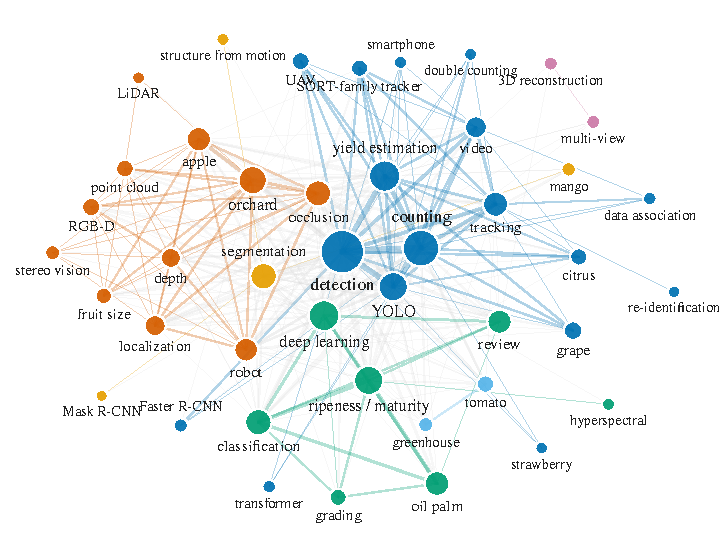
\includegraphics{F08_istilah}
\caption{Term co-occurrence map of the included studies, where node size, line width, and colour represent the number of studies containing the term in the title or abstract, the number of studies containing both terms, and the cluster, respectively.}\label{fig:terms}
\end{figure}

\section{Crops, platforms, and sensors of the method studies}\label{sup:landscape}

Fig.~\ref{fig:crop} relates crop to association mechanism. Apple accounts for \nCropApple of the \nMethod method studies, citrus for \nCropCitrus, grape for \nCropGrape, tomato for \nCropTomato, strawberry for \nCropStrawberry, and mango for \nCropMango.

Fig.~\ref{fig:sensor} gives modality and platform by crop. Crop and platform were read from the full text of each study: the crop whose fruit the study itself detected, counted, or tracked, and what carried the camera when its images were taken. Of the \nMethod method studies, \nPlatNone do not state the platform, \nPlatGround used a ground vehicle or robot, \nPlatUav an unmanned aerial vehicle (UAV), \nPlatHand a handheld device or smartphone, and \nPlatSeveral more than one platform; each study is counted once. Modality was coded by keyword rules from titles and abstracts: a red-green-blue (RGB) camera is the sensor in \nModRgb studies; RGB-D cameras appear in \nModRgbd, stereo cameras in \nModStereo, light detection and ranging (LiDAR) in \nModLidar, and multispectral cameras in \nModMulti. The modality counts depend on what is named in titles and abstracts and can omit sensors reported only in the full text.

\begin{figure}[ht]
\centering
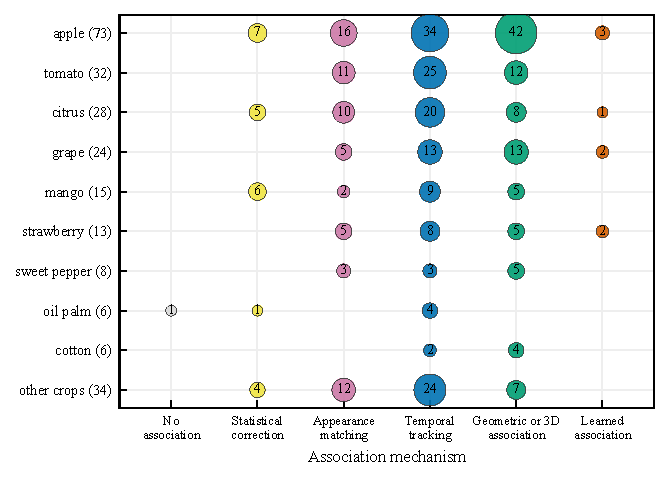
\includegraphics{F05_tanaman_mekanisme}
\caption{Multi-observation method studies by crop and association mechanism ($n=\nMethod$), where the number in each circle is the study count.}\label{fig:crop}
\end{figure}

\begin{figure}[ht]
\centering
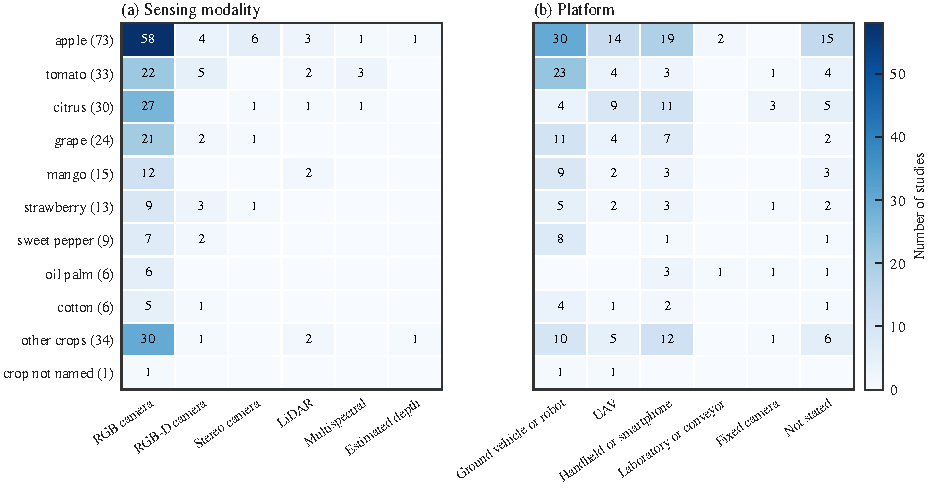
\includegraphics{F10_sensor}
\caption{Sensing modality and platform by crop in the multi-observation method studies ($n=\nMethod$): (a) modality; (b) platform.}\label{fig:sensor}
\end{figure}

\section{PRISMA 2020 checklist}\label{sup:prisma}

Table~\ref{tab:prisma} gives the location of each item of the PRISMA 2020 checklist \citep{page2021prisma} in the main article or in this supplement. Item texts are abbreviated. Items about pooled results are marked as not applicable because the review is a mapping review that does not pool effect sizes.

\begin{footnotesize}
\setlength{\tabcolsep}{3pt}
\begin{longtable}{@{}L{3.0cm}L{0.8cm}L{6.4cm}L{\dimexpr\linewidth-10.2cm-6\tabcolsep\relax}@{}}
\caption{PRISMA 2020 checklist with the location where each item is reported.}\label{tab:prisma}\\
\toprule
Section and topic & Item & Checklist item & Location\\
\midrule
\endfirsthead
\toprule
Section and topic & Item & Checklist item & Location\\
\midrule
\endhead
\bottomrule
\endfoot
Title & 1 & Identify the report as a systematic review. & Title\\
Abstract & 2 & Report the abstract according to the PRISMA 2020 for Abstracts checklist. & The abstract presents the objective, main findings, and implications. Section 2 reports eligibility, sources, appraisal, synthesis, and registration. Section 10 discusses limitations. Funding awaits author confirmation.\\
Introduction: rationale & 3 & Describe the rationale for the review in the context of existing knowledge. & Section 1; Section 9.3\\
Introduction: objectives & 4 & State the objectives or questions the review addresses. & Section 1, questions (1)--(4)\\
Methods: eligibility criteria & 5 & Specify the inclusion and exclusion criteria and how studies were grouped for the syntheses. & Sections 2.2 and 2.4; Section S7\\
Methods: information sources & 6 & Specify all sources searched or consulted and the date each was last searched. & Section 2.1 (Scopus, 28 September 2026); Section 2.3 and Section S1 (reference lists of the closest reviews)\\
Methods: search strategy & 7 & Present the full search strategies, including filters and limits. & Section S7; Appendix B\\
Methods: selection process & 8 & Specify how inclusion was decided: number of reviewers, independence, and automation tools. & Section 2.3; Section S1\\
Methods: data collection process & 9 & Specify how data were collected: number of reviewers, independence, and automation tools. & Section 2.4; Section S2; declaration of generative AI\\
Methods: data items & 10a & List and define the outcomes for which data were sought. & Sections 2.4 and 2.5; Section 5.6\\
 & 10b & List and define the other variables for which data were sought. & Section 2.4; Sections S2 and S4\\
Methods: risk of bias in studies & 11 & Specify the methods used to assess risk of bias in the included studies. & Section 2.5; Section S7. No formal study-level risk-of-bias tool was applied.\\
Methods: effect measures & 12 & Specify the effect measures used for each outcome. & Section 2.5: metrics as reported by each study; no pooled effect measure\\
Methods: synthesis methods & 13a & Describe how studies were selected for each synthesis. & Section 2.4 (groups); Section 2.5 (conditions for a comparison on the same data)\\
 & 13b & Describe any preparation of data for presentation or synthesis. & Section 2.5; notes to the acquisition and association tables\\
 & 13c & Describe how results were tabulated or displayed. & Sections 4--8; Sections S8 and S9\\
 & 13d & Describe the synthesis methods and their rationale. & Section 2 (configurative synthesis without pooling); Section 2.5 (structured narrative)\\
 & 13e & Describe methods used to explore heterogeneity among results. & Sections 4 and 5; Section S9\\
 & 13f & Describe any sensitivity analyses. & No formal sensitivity analysis of the synthesis was performed\\
Methods: reporting bias assessment & 14 & Describe methods used to assess the risk of bias due to missing results. & Not assessed; retrieval bias is discussed in Section 10\\
Methods: certainty assessment & 15 & Describe methods used to assess certainty in the body of evidence. & Section 2.5; Section S7\\
Results: study selection & 16a & Describe the results of the search and selection, ideally with a flow diagram. & Section 2.3; Fig.~1\\
 & 16b & Cite studies that might appear to meet the criteria but were excluded, and explain why. & Supplementary Data S1 (reports excluded at full text, with reasons); Section 2.3 (second reports of included studies)\\
Results: study characteristics & 17 & Cite each included study and present its characteristics. & Supplementary Data S1; Appendix Table A1; Sections S4 and S8\\
Results: risk of bias in studies & 18 & Present assessments of risk of bias for each included study. & No formal study-level risk-of-bias assessment. Sections 4 and 5 report the reference and outcomes of selected comparisons.\\
Results: individual studies & 19 & Present the results of each study for each outcome. & Selected comparisons in Sections 4--8 and S9; principal results of multi-observation reports in Appendix Table A1\\
Results: syntheses & 20a & Summarize the characteristics and risk of bias of the studies in each synthesis. & Sections 5.6 and 9.2; Sections S4 and S8\\
 & 20b & Present the results of all statistical syntheses. & No pooled statistical synthesis was performed.\\
 & 20c & Present the results of investigations of heterogeneity. & Sections 4 and 5; Section S9\\
 & 20d & Present the results of sensitivity analyses. & No formal sensitivity analysis of the synthesis was performed\\
Results: reporting biases & 21 & Present assessments of risk of bias due to missing results. & Not assessed; Section 10\\
Results: certainty of evidence & 22 & Present assessments of certainty in the body of evidence. & Certainty table in Section 9.2\\
Discussion & 23a & Provide a general interpretation of the results. & Section 9\\
 & 23b & Discuss limitations of the evidence included in the review. & Sections 5.6 and 9.4\\
 & 23c & Discuss limitations of the review processes used. & Section 10\\
 & 23d & Discuss implications for practice, policy, and future research. & Sections 9.4, 9.5, and 11\\
Other information: registration and protocol & 24a & Provide registration information or state that the review was not registered. & Section 2: not registered\\
 & 24b & Indicate where the protocol can be accessed or state that none was prepared. & Section 2 states that the review was unregistered. Sections S1 and S2 give screening and coding rules.\\
 & 24c & Describe and explain any amendments to the registration or protocol. & Not applicable; changes to codes made during verification are recorded in the change log (Section S6)\\
Other information: support & 25 & Describe sources of financial or non-financial support. & Funding\\
Other information: competing interests & 26 & Declare any competing interests of the review authors. & Declaration of competing interest\\
Other information: availability of data, code, and materials & 27 & Report which data, code, and materials are publicly available and where. & Data availability; Section S6\\
\end{longtable}
\end{footnotesize}

\section{Files provided}\label{sup:files}

Supplementary Data S1 (\texttt{main7-supplementary-studies.csv}) is a table in comma-separated values format with one row for each of the \nFTAssessed reports assessed in full text: the \nIncluded included studies, ordered by group, followed by the \nFTExcl reports excluded at the full-text stage. Its columns give the status (included or excluded at full text), the group, the reason for exclusion in the words of the flow diagram, the first author, year, title, source, and digital object identifier, the association mechanism and acquisition design of each multi-observation study, and whether the study is cited in the main article, including its appendices.

The screening decisions, coded evidence matrix, verification log, and scripts are part of the review data. The data availability statement in the main article identifies the materials.

\section{Search summary, evidence groups, and appraisal}\label{sup:appraisal}
Table~\ref{tab:queries} gives the query families, with complete strings and limits in Appendix B of the main article. Table~\ref{tab:groups} describes the seven mutually exclusive groups. The group determines how a report contributes to the synthesis. Full-text eligibility was assessed for all included reports, but detailed coding was specific to the group.

\begin{table}[htbp]
\centering
\caption{Scopus query sets and number of records returned and retained.}\label{tab:queries}
\footnotesize
\begin{tabularx}{\linewidth}{@{}L{2.5cm}Yrr@{}}
\toprule
Query set (key) & Search terms & Returned & Retained\\
\midrule
Multi-observation counting (Q1) & Fruit or crop terms AND counting or yield AND multi-view, video, tracking, SfM, SLAM, duplicates & 871 & 871\\
Counting in titles (Q2) & Fruit AND counting or load in the title & 757 & 757\\
Oil-palm imaging (Q3) & Oil palm or FFB AND imaging, learning, ripeness, or counting & 1{,}079 & 1{,}079\\
Class attributes with counting (Q4) & Fruit AND ripeness, grade, or class AND counting AND detection & 361 & 361\\
Depth and 3D sensing (Q5) & Fruit AND RGB-D, stereo, LiDAR, or point cloud AND detection or counting & 1{,}988 & 1{,}988\\
Reviews of association methods (Q6) & Reviews of MOT, re-ID, multi-view detection, SfM, SLAM & 236 & 236\\
Reviews of fruit detection and yield (Q7) & Reviews of fruit detection, counting, ripeness, yield & 1{,}049 & 1{,}049\\
Methods outside agriculture, five title searches (Q8a--Q8e) & MOT, multi-view, SfM/SLAM, object counting, re-ID in the title & 23{,}532 & 125\\
Named foundational methods (Q9) & Titles of named methods (SORT, NeRF, SAM, \dots) & 1{,}082 & 25\\
\midrule
Total & & & 6{,}491\\
\bottomrule
\multicolumn{4}{@{}p{\linewidth}@{}}{\rule{0pt}{2.6ex}\textit{Note:} Full strings are given in Appendix~B of the main article under the same keys. For the last two sets only the 25 most cited records of each search were retained. FFB, fresh fruit bunch; SfM, structure from motion; SLAM, simultaneous localization and mapping; MOT, multiple-object tracking; re-ID, re-identification; RGB-D, red-green-blue-depth; LiDAR, light detection and ranging; SORT, simple online and realtime tracking; NeRF, neural radiance field; SAM, Segment Anything Model.}
\end{tabularx}
\end{table}

\begin{table}[htbp]
\centering
\caption{Groups of included studies ($n=\nIncluded$).}\label{tab:groups}
\footnotesize
\begin{tabularx}{\textwidth}{@{}L{3.0cm}YrL{3.3cm}@{}}
\toprule
Group & Definition & Studies & How coded\\
\midrule
Multi-observation studies & Combine several observations of the same fruit (video, several views, or repeated scans) and count, estimate, map, or link fruit across images & \nMulti & Individual full-text coding\\
Single-view counting studies & Count fruit or estimate yield from single images & \nSingle & Descriptive keywords, spot-checked\\
Oil-palm studies & Image oil-palm fresh fruit bunches or loose fruit, including mill grading & \nPalm & Individual full-text coding\\
Single-image class-wise counting studies & Count fruit by class in single images & \nClassSingle & Descriptive keywords, spot-checked\\
Depth and 3D sensing studies & Detect, locate, or measure fruit with depth, 3D, or a non-RGB modality & \nDepth & Descriptive keywords, spot-checked\\
Earlier reviews & Review fruit detection, counting, yield estimation from images, or oil-palm imaging & \nReviews & Descriptive keywords and close reading of the closest reviews\\
Methods papers from outside agriculture & Tracking, re-identification, multi-view association, 3D reconstruction, or object counting & \nOutside & Descriptive keywords\\
\bottomrule
\end{tabularx}
\end{table}

\textit{Certainty of individual findings.} Numerical contrasts used the same test images, videos, or plants, reported a value for each arm, and varied a choice in acquisition or association. The unsuccessful depth-assisted background removal described by \citet{garderes2024apple} supplied qualitative opposing evidence for the depth finding. It has no paired numerical outcome. The grading treated studies from one research group or using the same data as one group. High certainty required support from at least three groups on at least two crops, no group opposing the finding, at least one supporting field reference (harvest, packhouse, or hand count on the plant), and at least one supporting comparison favouring a method other than the authors' own. Moderate certainty required at least two supporting groups without opposition, or at least three with no more than one group opposing the finding. Other findings were graded low. Mixed results are retained in the evidence table. These grades characterize the support for each finding within the available evidence.

\section{Quantitative profile of the mapped studies}\label{sec:landscape}
Fig.~\ref{fig:tahun} gives the year and evidence group of the \nIncluded studies. The 2027 issue entry was available online before the search date.

\begin{figure}[htbp]
\centering
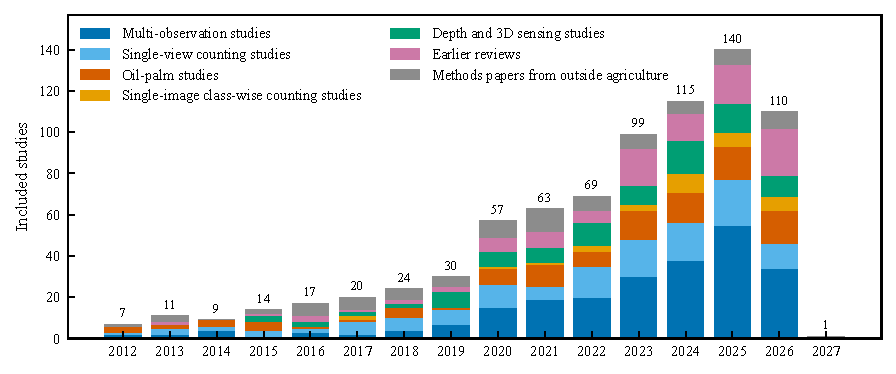
\includegraphics{F02_tahun}
\caption{Number of included studies per year by group ($n=\nIncluded$); studies for 2026 cover the period up to the search date, and the study for 2027 is a review published online before that date.}\label{fig:tahun}
\end{figure}

Of the \nMulti multi-observation studies, \nMultiData are dataset papers and \nMethod propose or evaluate a method; the statistics below refer to these \nMethod studies, and their crops, platforms, and sensors are given in Supplementary Section~S4. Because a study may combine mechanisms, mechanism values are occurrences.

\textit{(i) Temporal tracking has become more common in the mapped literature.} Temporal tracking appears in \nTrack of the \nMethod studies (\pTrack\%), geometric association in \nGeom (\pGeom\%), appearance matching in \nApp (\pApp\%), statistical correction in \nStat (\pStat\%), learned association in \nLearn, and no association in \nNone (Fig.~\ref{fig:mek}a). Of the \nEarly studies published before 2018, \nEarlyGeom used geometric association, \nEarlyStat statistical correction, and \nEarlyTrack temporal tracking; since 2023, temporal tracking has appeared in \pTrackRecent\% of the \nRecent new studies, and appearance matching, mostly inside trackers that carry an appearance descriptor, in \pAppRecent\%.

\textit{(ii) Acquisition is mostly video.} Of these studies, \nVideo acquire video along a path, \nDiscrete use discrete views, \nScan use 3D scans, and \nRevisit revisit the same plants over time (Fig.~\ref{fig:mek}b). Acquisition and mechanism are coupled (Fig.~\ref{fig:flow}): video feeds temporal tracking alone (\nTrackOnly studies), appearance matching combined with tracking (\nAppTrack), and tracking combined with geometric association (\nTrackGeomVideo; another \nTrackGeomScan combine the two on 3D scans), whereas among the \nDiscrete studies with discrete views, geometric association appears in \nDiscreteGeom and statistical correction in \nDiscreteStat.

\textit{(iii) Classes are rarely counted on unique fruit.} Only \nPerClass of the \nMethod studies report counts per class (Section~6 of the main article).

\begin{figure}[htbp]
\centering
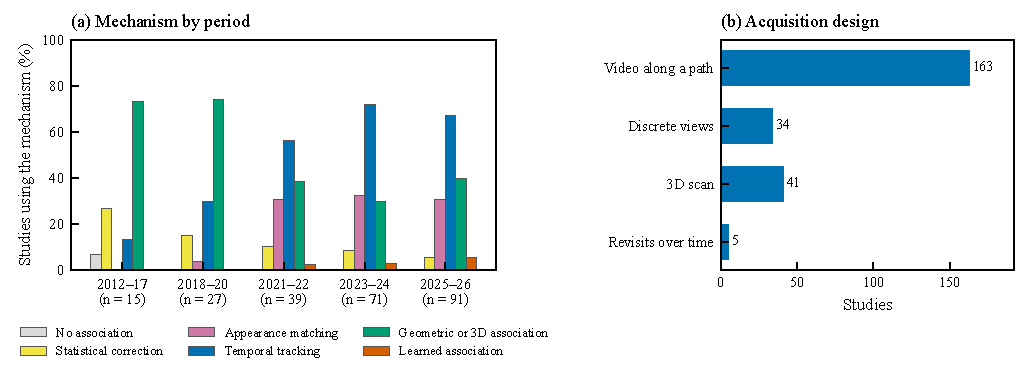
\includegraphics{F04_mekanisme}
\caption{Association mechanisms and acquisition design in the multi-observation method studies ($n=\nMethod$): (a) share of studies using each mechanism by period; (b) acquisition design.}\label{fig:mek}
\end{figure}

\begin{figure}[htbp]
\centering
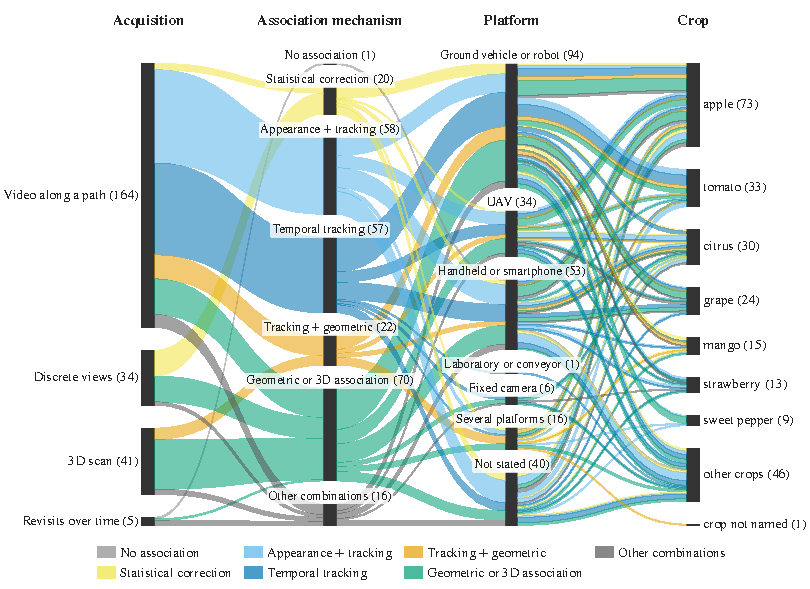
\includegraphics{F09_alur}
\caption{Acquisition design, association mechanism, platform, and crop of the multi-observation method studies ($n=\nMethod$), where each study is placed in one category, so a single mechanism name means that mechanism alone, and band width and colour represent study count and mechanism, respectively.}\label{fig:flow}
\end{figure}

\subsection{Oil-palm imaging}
Fig.~\ref{fig:sawit} displays the tasks and acquisition settings in the oil-palm group. The figure distinguishes reports that count fruit or bunches in images from those that use multiple views. The multiple-view label records acquisition and does not imply that fruit identities were linked.

\begin{figure}[htbp]
\centering
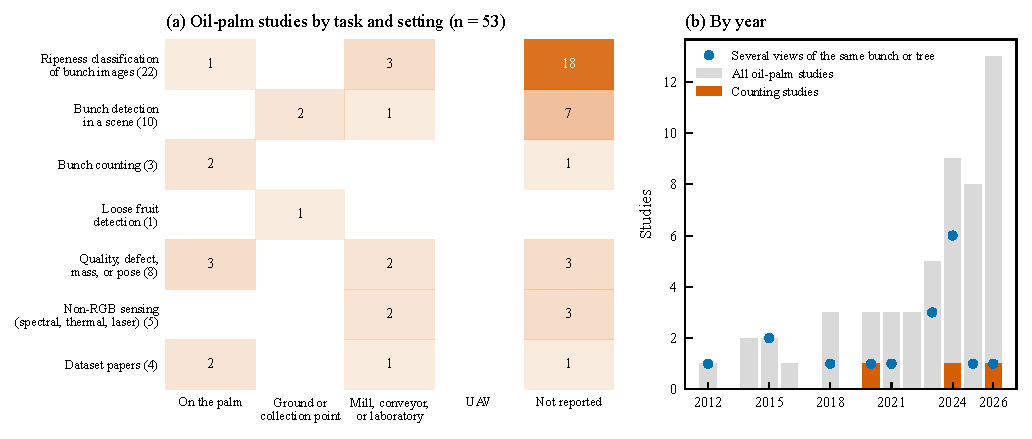
\includegraphics{F06_sawit}
\caption{Oil-palm studies ($n=\nPalm$): (a) task by setting; (b) studies per year, with counting studies and studies that use several views marked.}\label{fig:sawit}
\end{figure}

\section{Comparison record}\label{sup:comparisons}

Table~\ref{tab:comparison-register} records which studies found gains, losses, or mixed results when a component was changed on the same test data. The direction is based on the reported outcomes. Several entries involve changes to more than one system component, and some reports share test data. The main article reports representative numerical contrasts with their references, and the appraisal treats reports using the same data or coming from the same research group as one source of support.

\begin{footnotesize}
\setlength{\tabcolsep}{4pt}
\begin{longtable}{@{}L{2.8cm}L{3.6cm}L{3.5cm}L{5.0cm}@{}}
\caption{Reported directions of comparisons on the same data, grouped by the component varied.}\label{tab:comparison-register}\\
\toprule
What was varied & Varied element improved the result & Did not improve, or mixed & What the direction depended on\\
\midrule
\endfirsthead
\toprule
What was varied & Varied element improved the result & Did not improve, or mixed & What the direction depended on\\
\midrule
\endhead
\bottomrule
\endfoot
(1) Generic appearance descriptor (DeepSORT, StrongSORT; \citealp{wojke2017simple,du2023strongsort}) against motion matching (SORT) & \citet{vaishnavi2025fruit}; \citet{si2026citrus}; \citet{villacres2023apple}; \citet{piazolo2026enhanced}; \citet{poncemachete2025optimizing}; \citet{an2024stratracker}; \citet{feng2026greenhouse}; \citet{zhai2025dynamic} & \citet{zhang2022deep}; \citet{genemola2023video}; \citet{weng2026citrus} & Missed detections: with annotated boxes removed at random until 60\% remained, DeepSORT kept MOTA at 69.3\% and SORT fell to 13.8\% \citep{villacres2023apple}; on apples, the authors attributed the absence of a gain to the similar appearance of the fruit \citep{genemola2023video}\\
\addlinespace
(2) Generic appearance descriptor against a tracker that keeps low-confidence boxes (ByteTrack) & \citet{pai2024maturity}; \citet{an2024stratracker}; \citet{piazolo2026enhanced}; \citet{zhou2024advancing}; \citet{zhai2025dynamic} & \citet{genemola2023video}; \citet{poncemachete2025optimizing}; \citet{sekharamantry2024seamless}; \citet{huang2026mfft}; \citet{wu2025maturity}; \citet{weng2026citrus}; \citet{felippomes2026video}; \citet{feng2026greenhouse}; reversed by metric or rule: \citet{qi2025assessment}; \citet{zhang2025row} & The two address different failures: the descriptor re-links a fruit after it was lost, whereas ByteTrack keeps partly occluded fruit from being lost; the ranking reversed between identity and count metrics \citep{qi2025assessment} and with the counting rule \citep{zhang2025row}, and one study attributed the weak ByteTrack result to the absence of parameter tuning \citep{zhou2024advancing}\\
\addlinespace
(3) Camera-motion compensation added, or BoT-SORT against ByteTrack & \citet{zhang2024stablesort}; \citet{saraceni2024agrisort}; \citet{huang2019high}; \citet{felippomes2026video}; \citet{kemper2025performance}; \citet{zhai2025dynamic}; \citet{an2024stratracker} & \citet{zhou2024utilizing}; \citet{weng2026citrus}; \citet{feng2026greenhouse}; mixed: \citet{wei2025multi} & Gains came from platforms that shake or turn, such as a legged robot, and from rough vineyard terrain; BoT-SORT also changes the motion filter and may add a descriptor, so its rows do not isolate the compensation; one reversal used surround video recorded at constant speed\\
\addlinespace
(4) A cue built by the authors (fruit-specific appearance, position, or platform motion) added to a tracker & \citet{kirk2021robust}; \citet{yang2024automatic}; \citet{dong2025fruit}; \citet{meng2024real}; \citet{hu2023fruit}; \citet{du2024green}; \citet{ahmedtaristizabal2024field}; \citet{zheng2023object}; \citet{lei2025spatio}; \citet{dai2022tracking}; \citet{piazolo2026enhanced} & Mixed across matching settings: \citet{fusaro2026horticultural} & Each cue was tested only by its own authors, except a histogram descriptor from earlier work, which two other groups re-implemented and which lost in both \citep{fusaro2026horticultural,lei2025spatio}; gains ranged from 1.1 points of MOTA \citep{dong2025fruit} to a reduction in count error from 41 to 7 strawberries \citep{kirk2021robust}\\
\addlinespace
(5) Geometric or 3D step after tracking or summation & \citet{liu2018robust}; \citet{gongal2016apple}; \citet{wei2025multi}; \citet{santos2024multiple}; \citet{matos2024tracking}; \citet{ciarfuglia2023weakly}; \citet{zhou2024utilizing}; \citet{yoshida2026cross} & Mixed on shared apple data: \citet{hani2020comparative}; \citet{roy2019vision}; \citet{dong2020semantic} & A common frame can remove overlap between opposite sides. On one apple dataset, the unmerged GMM-based sum was closer to the harvest count than the merged result. With annotated citrus boxes, 3D relocalization raised HOTA from 0.434 to 0.935 \citep{santos2024multiple}. See Section~5.4 of the main article.\\
\addlinespace
(6) Counting rule & A rule that uses track history outperformed a raw identity count or one line: \citet{zhou2024advancing}; \citet{zhang2025row}; \citet{zheng2023efficient}; \citet{rong2023tomato}; \citet{tenorio2021automatic}; \citet{an2024stratracker}; \citet{feng2026greenhouse}; \citet{lu2025iot} & Counting every identity outperformed one counting line: \citet{parico2021real}; \citet{sasse2025object} & The rule reordered trackers in strawberry and kiwifruit video and detector--tracker pairs in citrus video \citep{zhou2024advancing,zhang2025row,zheng2023efficient}. In the apple comparison, tracks shorter than five detections were removed from the reference as well as the predictions \citep{matos2024tracking}.\\
\addlinespace
(7) Statistical correction of a raw count & Factor fitted on the same block or dataset: \citet{wang2013automated}; \citet{indriani2026sawitmvc} & Factor transferred from calibration trees: \citet{anderson2021estimation} & Whether the factor was fitted where it was applied: in-sample factors brought row errors from $-29.8$\% and $-41.3$\% to 1.8\% and 0.4\% \citep{wang2013automated}, whereas a factor from hand-counted trees raised the absolute percentage error against packhouse counts from 11\% to 17\% \citep{anderson2021estimation}\\
\addlinespace
(8) Linking observations against summing per-frame detections & \citet{hu2023fruit}; \citet{louis2025automated} & None found & Summing retains detections in each frame. The sum was 495 against a manual video count of 290. Tracking returned 310 \citep{hu2023fruit}\\
\end{longtable}
\end{footnotesize}

\section{Scope of closely related reviews}

Table~\ref{tab:position} compares the organizing questions and search descriptions of the reviews closest in scope to the present analysis. It records the stated methods so that coverage claims can be interpreted in light of each review's scope.

\begin{footnotesize}
\begin{longtable}{@{}L{2.7cm}L{\dimexpr\textwidth-9.2cm-6\tabcolsep\relax}L{3.4cm}L{3.1cm}@{}}
\caption{Earlier reviews closest to this review ($n=17$).}\label{tab:position}\\
\toprule
Review & Scope & Organizing variable & Stated method\\
\midrule
\endfirsthead
\toprule
Review & Scope & Organizing variable & Stated method\\
\midrule
\endhead
\bottomrule
\endfoot
\bottomrule
\multicolumn{4}{@{}p{\textwidth}@{}}{\rule{0pt}{2.6ex}\textit{Note:} Not stated indicates that the report does not describe how sources were identified. PRISMA, Preferred Reporting Items for Systematic Reviews and Meta-Analyses.}\\
\endlastfoot
\citet{gongal2015sensors} & Machine vision for fruit detection and localization in robotic harvesting and crop-load estimation & Sensor type, image features, classifier, and localization method & Not stated\\
\citet{koirala2019deepb} & Deep learning for fruit detection and yield estimation & Detection framework, training, evaluation, and architecture & Not stated\\
\citet{anderson2021technologies} & Forecasting fruit load and harvest timing in tree crops & Estimation route (sampling, vision, remote sensing, models, harvest timing) & Literature base described by Scopus keyword counts; no selection procedure\\
\citet{maheswari2021intelligent} & Semantic segmentation for fruit yield estimation in orchards & Workflow stage and network architecture & Not stated\\
\citet{barriguinha2021vineyard} & Vineyard yield estimation, prediction, and forecasting & Methodological approach (ten groups) & Six databases, PRISMA as a guideline; 82 of 455 records included\\
\citet{he2022fruit} & Pre-harvest orchard yield prediction and estimation & Indirect prediction against direct estimation, by platform and model & Five databases, journal articles 2010--2021, stated exclusion criteria\\
\citet{mohimont2022computer} & Computer vision with RGB images in viticulture & Task (flower, bunch, and berry detection; yield estimation) & Not stated\\
\citet{huang2023survey} & Deep-learning object detection for crop counting & Counting method (manual, image processing, density regression, segmentation, detection) and detector architecture & Three keyword strings in Google Scholar, ScienceDirect, and IEEE Xplore, 2019--2023, plus citation tracking; numbers not stated\\
\citet{miranda2023fruit} & In-field fruit sizing, detection, counting, and maturity estimation & Task (detection, tracking and counting, sizing from 2D and 3D data, maturity) & Not stated\\
\citet{magro2023computational} & Yield estimation and forecasting models for perennial fruit crops & Assessment strategy, model class, and input variables & Three databases, title and abstract screening; 49 articles\\
\citet{rong2026research} & Orchard yield estimation with multi-source information & Technical approach (manual, machine vision, remote sensing, learning) & Six databases and reference lists; about 436 records identified, number included not stated\\
\citet{liu2026shaping} & Citrus yield prediction & Prediction horizon, sensor platform, model type, region, spatial scale, and metrics & Scopus, 2005--2026, PRISMA~2020; 273 of 1{,}007 records selected\\
\citet{khan2021oil} & Machine learning in oil palm, 2011--2020 & Task (regression, classification) & Five databases; 61 papers after full-text screening\\
\citet{lai2023oil} & Oil-palm fresh-fruit-bunch ripeness detection & Sensing modality and classifier & Google Scholar keyword search; 51 papers in the abstract, 48 in the discussion\\
\citet{kamal2024machine} & Machine-learning maturity grading of oil-palm fruit & Processing stage (pre-processing, segmentation, features, classifier) & Self-described systematic; no databases or search strings reported\\
\citet{goh2025fresh} & Non-destructive ripeness classification of oil-palm fresh fruit bunches & Sensing technique & Self-described systematic; no databases or search strings reported\\
\citet{gunawan2026drone} & Drone- and deep-learning-based palm-fruit detection and yield measurement in Malaysia, Indonesia, and Thailand & Sensor payload, measurement chain, and country & Not stated\\
\midrule
This review & Turning repeated fruit observations into unique, class-labelled records; oil palm as the main case & Association mechanism and its assumptions & Systematic map, Scopus, PRISMA~2020; \nIncluded studies after full-text assessment\\
\end{longtable}
\end{footnotesize}

\bibliographystyle{cas-model2-names}
\bibliography{references6}
\end{document}
